\hypertarget{highly-overlapped-signals}{%
\chapter{Highly Overlapped Signals}\label{cha:highly-overlapped-signals}}

In the previous chapter, I introduced signal processing fundamentals in the context of audio mixtures.
In this chapter, I focus on scenarios of highly overlapped signals.
To formalize the \emph{level of overlap}, a time-frequency representation as introduced in Section~\ref{sub:time-frequency-representation} and how they are typically applied to address the source separation problem.

\hypertarget{separability-of-mixtures}{%
\section{Separability of Mixtures}\label{separability-of-mixtures}}

Time-frequency representations such as the short-time Fourier transform (STFT) have clear benefits such as the improved interpretability due to its ``image-like'' two-dimensional properties.
More importantly, however, such a representation allows to separate mixtures of speech and musical instruments.
The reason for this is that these mixtures may be fully overlapped in the time domain but are less overlapped in the frequency domain~\cite{rickard02, giannoulis11, rafii}.
In turn, a TF representation allows applying to filter in a way that sufficiently extracts all targets from the mixture.
Furthermore, it allows for the reconstruction of the original waveform and provides a good trade-off between computational complexity and separation quality.
\par
Due to these reasons, many source separation methods focus on extracting individual sources by modeling their respective target in the time-frequency domain.
Further it is assumed that the STFT provides sufficient level of separability.
The actual extraction or filtering is done by synthesizing the magnitude estimate of the model and applying the originals mixture phase.
\par
In practice, the ability to extract a source from a mixture, depends on the amount of overlap between sources.
Without any overlap, separation is obviously not necessary, and a small amount of overlap can be tolerated to still sufficiently extract the sources.
However, if sources are fully overlapped in both, time and frequency, a separation in the TF domain is hardly possible.
A metric that is often used for the purpose of evaluation is called \emph{separability} and was found by Rickard in~\cite{rickard02} as a useful metric for both, speech and music~\cite{giannoulis11} signals.
\par
In linear mixtures, separability is defined as \emph{a measure that indicates the percentage of time-frequency bins of a source is disjoint from those of interfering sources}.
If \(M\) is the ideal binary mask for a given target \(S\) and it's interfering
magnitude model \(Y\), the W-disjoint orthogonality metric \(WDO\) is defined as:

\begin{equation}
    PSR_{M} = \frac{\|M \cdot S_{k}\|^{2}}{\|S_{k}\|^{2}}
\end{equation}

\begin{equation}
    SIR_{M}=\frac{\|M \cdot S_{k}\|^{2}}{\|M \cdot Y_{k}\|^{2}}
\end{equation}

\begin{equation}
    WDO_{M} = PSR_{M} - \frac{PSR_{M}}{SIR_{M}}
\end{equation}

A \(WDO\) of one means the sources are perfectly disjoint, hence no overlap.
A \(WDO\) zero means can be interpreted as sources being fully overlapped.
An extensive study using this W-disjoint orthogonality metric (WDO) is given in~\cite{rickard02}.
\par
The ability to separate sources is depending on the scenario and its applications.
Two scenarios that are very popular among research are:

\begin{description}
  \item[Cocktail Party] where multiple speakers are speaking concurrently, it results in an overlap of speech signals in both time an frequency. 
  \item[Vocals and Accompaniment] are often active at the same time in professionally produced music.
\end{description}

Now, for both scenarios, the actual overlap depends on additional parameters like the number of sources, the class of source or the fundamental frequency.
For instance, the overlap in a cocktail party of two speakers is smaller than with ten concurrent speakers speaking.
Also, the overlap between male and female or brass and string instruments is smaller than with two instruments of the same class. 
And if two instrumental notes share the same fundamental frequency (playing in \emph{unison}), the sources are almost entirely overlapped.
\par
\begin{figure*}[h]
\centering
\subcaptionbox[Speech]{Speech}%
[1\textwidth]{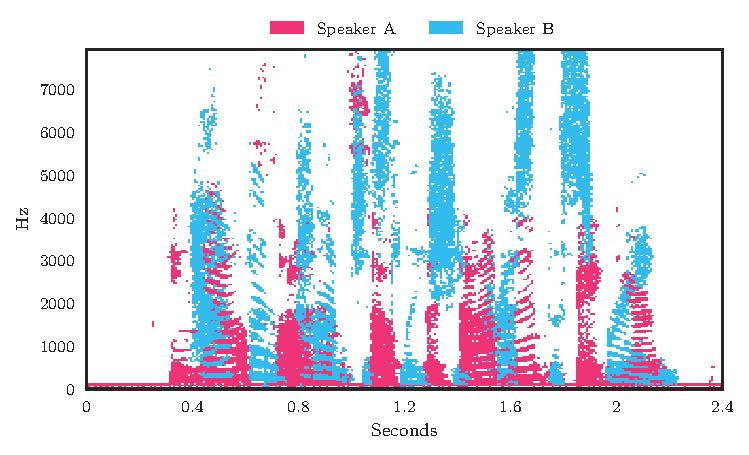
\includegraphics[width=0.8\textwidth]{gfx/dominance_map_speakers.pdf}}%
\hspace{0.2\textwidth} % seperation
\subcaptionbox[Vocal/Accompaniment]{Vocal/Accompaniment}
[1\textwidth]{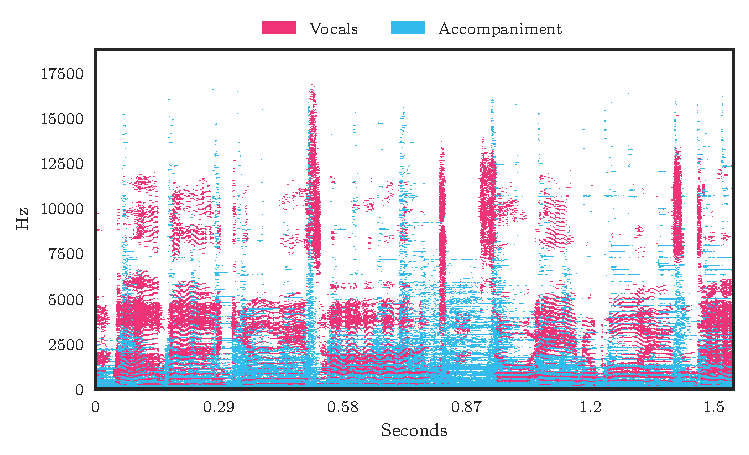
\includegraphics[width=0.8\textwidth]{gfx/dominance_map_vocacc.pdf}}%
\hspace{0.2\textwidth} % seperation
\subcaptionbox[Speech]{Unsison}
[1\textwidth]{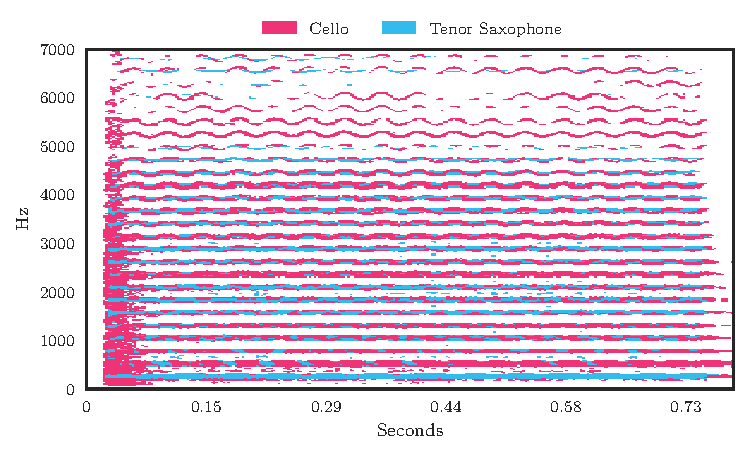
\includegraphics[width=0.8\textwidth]{gfx/dominance_map_unison.pdf}}%
\caption{Predominant source activity, showing the predominant source for each time frequency entry. Computed using binary masks of each source entry.}
\label{fig:dominance}
\end{figure*}

\begin{figure*}[h]
\centering
\subcaptionbox[Speech]{Speech}%
[1\textwidth]{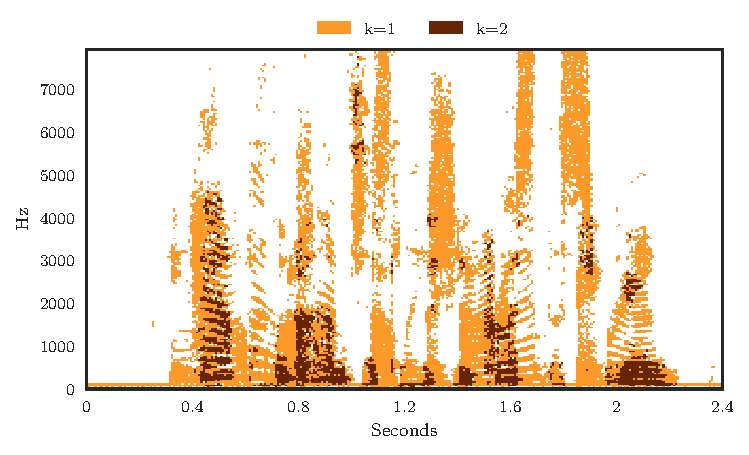
\includegraphics[width=0.8\textwidth]{gfx/count_map_speakers.pdf}}%
\hspace{0.2\textwidth} % seperation
\subcaptionbox[Vocal/Accompaniment]{Vocal/Accompaniment}
[1\textwidth]{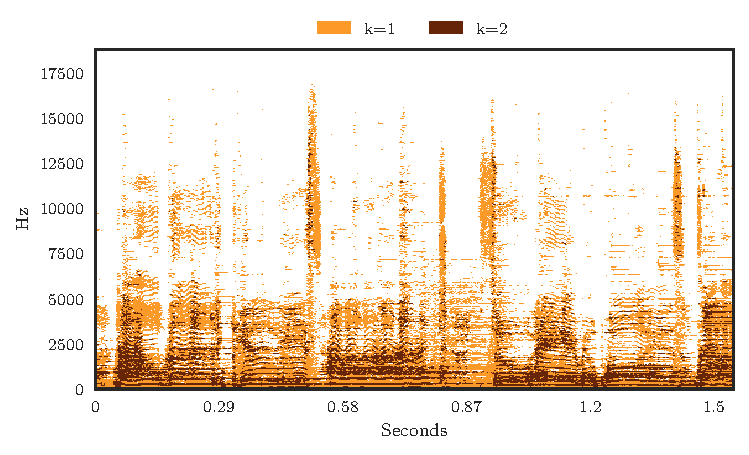
\includegraphics[width=0.8\textwidth]{gfx/count_map_vocacc.pdf}}%
\hspace{0.2\textwidth} % seperation
\subcaptionbox[Unison]{Unison Instruments}
[1\textwidth]{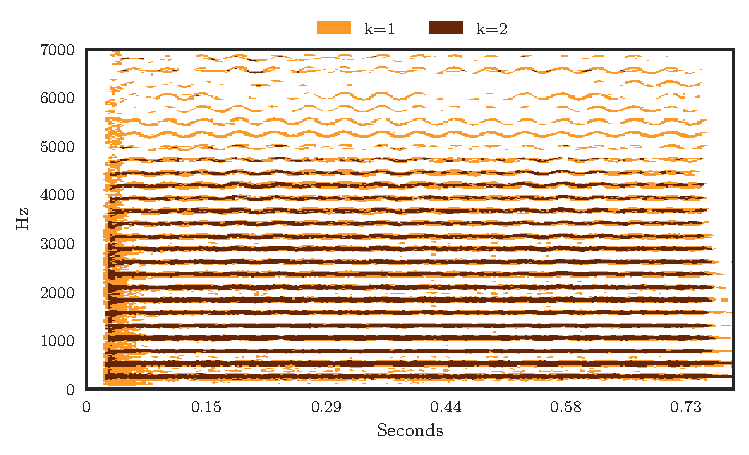
\includegraphics[width=0.8\textwidth]{gfx/count_map_unison.pdf}}%
\caption{Source Count Activity showing the number of sources $k$ for each time frequency entry. Computed using binary masks of each source entry.}
\label{fig:count}
\end{figure*}

To illustrate this, we depict the different scenarios in two figures.
Figure~\ref{fig:dominance} assigns each time-frequency entry that their predominant source classes.
Figure~\ref{fig:count} depicts the number of active sources of each TF entry.
From these figures, one can see that the overlap of a typical speech mixture is comparable to a music recording where the task is to separate vocals and accompaniment.
If we now compare this to the scenario where sources are fully overlapped as in the unison scenario, almost all TF bins are overlapped, and separation would hardly be possible.
\par
While this is an extreme scenario, it still provides a useful example where common assumptions are violated, and it would facilitate the demand to develop new methods that do not rely so much on these long-standing assumptions.
A naïve method can be developed by just observing the time-frequency representation in Figure~\ref{fig:count} closely.
We see that the slow spectro-temporal modulations caused by the vibrato are one of the aspects where the two sources differ significantly.
So here, the classical STFT does provide enough separability and representations as in the \emph{modulation spectrogram}, presented by~\cite{greenberg96} may be preferable.
Details about this approach are discussed in Chapter~\ref{cha:unknown}.

\hypertarget{exploiting-slow-modulations}{%
\section{Exploiting Slow Modulations}\label{exploiting-slow-modulations}}

Tempo-spectral modulations occur both in speech and music signals as detailed in Section~\ref{sub:time-variant-audio-signals}).
Exploiting modulations is natural for humans: early research from Zwicker in 1952 focused on the human ability to detect amplitude modulations~\cite{zwicker52}. 
Later, it was shown by Bregman, McAdams, and Fastl in~\cite{mcadams89, bregman90, fastl90} that humans use amplitude modulations to group sources; this concept was called \emph{Common Amplitude Modulation} (CAM).
CAM exploits the fact that harmonics share the same amplitude modulation across frequency bins, are perceived \emph{integrated} as opposed to~\emph{segregated}.
Further, it was shown in~\cite{bacon89} that the ability to detect amplitude modulations can be incorporated into auditory models.
It was then found by Dau in~\cite{dau99}; humans are especially sensitive at low-frequency modulations:

\begin{quote}
``Slow modulations are associated with the perception of rhythm. Samples of running speech, for example, show distributions of modulation frequencies with peaks around 3-4 Hz, approximately corresponding to the sequence rate of syllables~\cite{plomp83}. Results from physiological studies have shown that, at least in mammals, the auditory cortex seems to be limited in its ability to follow fast temporal changes.''
\end{quote}

Dau then proposed a model that mimics the ability to detect modulation patterns and pointed out applications to improve the perception for hearing-impaired listener or speech intelligibility.
\par
Previously, research has addressed a variety of tasks of processing and analysis in the context of modulations.
In the following, we give an overview of existing work focussed on analysis and separation of modulated sounds.

\subsection{Analysis}

Modulations play an essential role in various audio analysis tasks.
%lets start with speech
In speech techniques to utilize modulation patterns improved applications such as speech, discrimination~\cite{mesgarani04} or extract spatial acoustic signatures from mixtures~\cite{sukittanon06}.
One way of analyzing amplitude modulations is to use a modulation spectrogram~\cite{greenberg97} which is a frequency-frequency representation of a time domain input signal.
A complete signal representation can be archived by a modulation tensor which holds the modulation spectrograms for each time frame.
Interestingly, Greenberg assumed that ``the energy in the modulation spectrum may be derived from syllabic segmentation'' and that ``the preservation of the portion of the modulation spectrum between 2 and 10 Hz''.
Following this, it was later proved that the detection of modulations could improve speech intelligibility~\cite{elhilali03} or automatic speech recognition~\cite{kingsbury98}.
\par
% go to music
Amplitude modulations were also proposed for music tasks. 
Work by Scheirer in~\cite{scheirer99} proposed a method that operates by utilizing common modulation among groups of frequency sub-bands in the auto correlogram domain.
In music, predominantly caused by vibrato, amplitude modulations are considered to be that important, and the reader is referred to~\cite{muller11} for further details.
\par
A common way to explicitly analyze frequency variations is first to analyze the fundamental frequency and then track the fundamental frequency over time. 
An overview of various techniques is summarized in~\cite{driedger16}.
The authors of this paper also proposed a novel method to directly estimate the parameters of potential frequency modulations in the time-frequency domain by matching sinusoidal templates.
\par
For time-varying frequency modulations, the modulation spectrogram is not effective, as it would only be able to track the modulation rate due to the side-lobes of the modulation.
Disch and Edler proposed in~\cite{disch09} to decompose an audio signal into bandpass signals and each of them parametrically modeled by a sinusoidal carrier and its amplitude and frequency modulation.

\subsection{Processing}

As described in the previous chapter, modulations are used by humans to group and segregate sounds. Viste et al. describes the impact of modulation in~\cite{viste03} as:

\begin{quote}
``harmonic relation, the common onset, offset, amplitude modulation (AM), and frequency modulation (FM). These are all important cues for grouping.''
\end{quote}

\marginpar{This subsection is based on the work that has been published in~\cite{rafii}}

It is therefore not surprising that a number of methods exist, that utilize spectro-temporal modulations to separate mixtures.
% from zafar!
Wang proposed instantaneous and frequency-warped techniques for signal parameterization and source separation, with application to voice separation in music~\cite{wang94,wang95}.
He introduced a frequency-locked loop algorithm which uses multiple harmonically constrained trackers.
He computed the estimated fundamental frequency from a maximum-likelihood weighting of the tracking estimates. He was then able to estimate harmonic signals such as voices from complex mixtures.\\
% from zafar
The concept of \emph{common amplitude modulation} by~\cite{bregman, wang06} which exploits that amplitude envelopes of different harmonics of the same source tend to be similar.
Modeling the common amplitude modulation to separate mixtures has already been done in~\cite{li07, li09} and \cite{cano14}, which additionally included common amplitude modulation characteristics in the separation scheme.
% from zafar
Wolf et al. proposed an approach using rigid motion segmentation, with application to singing voice separation \cite{wolf14, wolf16}. They introduced harmonic template models with amplitude and pitch modulations defined by a velocity vector. They applied a wavelet transform \cite{anden14} on the harmonic template models to build an audio image where the amplitude and pitch dynamics can be separated through the velocity vector. They then derived a velocity equation, similar to the optical flow velocity equation used in images \cite{bernard01}, to segment velocity components. Finally, they identified the harmonic templates which model different sources in the mixture and separated them by approximating the velocity field over the corresponding harmonic template models.\\
% from zafar
Yen et al. proposed an approach using spectro-temporal modulation features \cite{yen14,yen15}. They decomposed a mixture using a two-stage auditory model which consists of a cochlear module \cite{chi05} and cortical module \cite{chi99}. They then extracted spectro-temporal modulation features from the TF units and clustered the TF units into harmonic, percussive, and vocal components using the EM algorithm and re-synthesized the estimated signals.\\
% from zafar
% double check this!
Virtanen made us of sinusoidal modeling \cite{virtanen00} to model and separate sources with tempo spectral modulation like vibrato.

In another vein, the source-filter model was deployed to separation sources~\cite{hennequin10}.
An advantage of the source-filter model approach is indeed that one can dissociate the pitched content of the signal, embodied by the position of its harmonics, from its TF envelope which describes where the energy of the sound lies. In the case of vocals, it yields the ability to distinguish between the actual note being sung (pitch content) and the phoneme being uttered (mouth and vocal tract configuration), respectively. 
One key feature of vocals is they typically exhibit great variability in fundamental frequency over time. 
They can also exhibit larger \textit{vibratos} and \textit{tremolos} in comparison to other instruments.

\section{Summary}

Modulations play an essential role in audio signals. 
However past research was mainly focused on single notes and not on overlapped sounds.
It is, therefore, to be investigated if scenarios with severe overlap can utilize modulations as well: Firstly, parameterization of modulation characteristics of a single source is difficult, when only the mixture can be observed. 
It is known~\cite{salamon13} that the extraction of the fundamental frequency in a mixture is challenging. 
The reason is that crossing partials are a challenging problem for sinusoidal modeling~\cite{viste03}. 
And even if tracking of them would work correctly, evaluation of robustness and accuracy is often hardly possible when the reference data is annotated with human precision.
Secondly, representations like modulation spectrograms only cover amplitude modulations, whereas general modulation patterns (AM/FM, timbre modulation) cannot be covered.
\par
In the last chapter, we showed the importance of modulations and in the next two chapters address this questions by utilizing the modulations of sources for separation tasks; either via prior knowledge (known) or by operating blindly (unknown).

\begin{itemize}
  \item Can modulations be automatically detected or extracted from highly overlapped signals?
  \item If modulations are known, can they be exploited to improve a task such as source separation?
  \item Can modulations still be utilized when modulation function and its cause of modulation is unknown?
  \item What is the role of modulations in the task of count estimation?
\end{itemize}


